\documentclass[tikz]{standalone}
\usepackage{amsmath}

\begin{document}

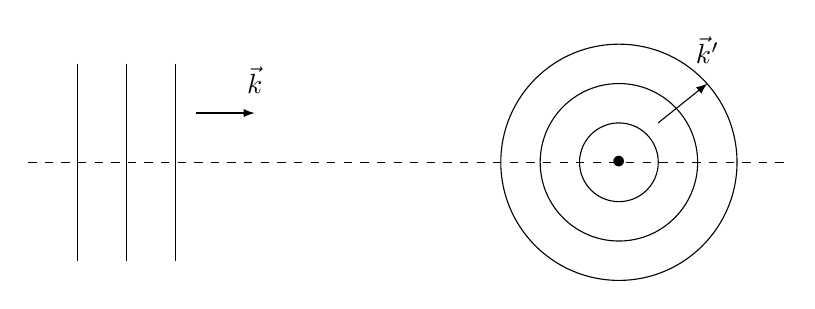
\begin{tikzpicture}[scale=1.25]
    \draw (0,0) -- (0,-2);
    \draw (0.5,0) -- (0.5,-2);
    \draw (1,0) -- (1,-2);
    \draw [-latex] (1.2,-0.5)-- (1.8,-0.5) node [label=above:{$\Vec{k}$}] {};
    \node (a) at (5.5,-1) {$\bullet$}; 
    \draw[black] (a) circle (0.4);
    \draw[black] (a) circle (0.8);
    \draw[black] (a) circle (1.2);
    \draw[dashed] (-0.5,-1) -- (7.2,-1);
    \draw [-latex] (5.9,-0.6)-- (6.4,-0.2) node [label=above:{$\Vec{k}'$}] {};
    \end{tikzpicture}

\end{document}